\newpage
\addcontentsline{toc}{chapter}{\textbf{Appendices}}

\addcontentsline{toc}{section}{A: Supplemental material for ``Root mass carbon costs to acquire nitrogen are determined by nitrogen and light availability in two species with different nitrogen acquisition strategies''}
\begin{center}
    \noindent \textbf{Appendices}
\end{center}
\begin{center}
    \noindent \textbf{Appendix A}
\end{center}
\begin{center}
    \begin{singlespace}
        \textbf{Supplemental material for ``Structural carbon costs to acquire nitrogen are determined by nitrogen and light availability in two species with different nitrogen acquisition strategies''}
    \end{singlespace}
\end{center}


\setcounter{table}{0}
\renewcommand{\thetable}{A\arabic{table}}

\setcounter{figure}{0}
\renewcommand{\thefigure}{A\arabic{figure}}

\begin{table}[h!]
    \caption[Summary table containing volumes of compounds used to create modified Hoagland's solutions for each soil nitrogen fertilization treatment]{Summary table containing volumes of compounds used to create modified Hoagland's solutions for each soil nitrogen fertilization treatment. All volumes are expressed as milliliters per liter (mL L$^{-1}$)}
    \label{table:tab.a1}
    \resizebox{\columnwidth}{!}{%
    \begin{tabular}{p{4cm}p{2cm}p{2cm}p{2cm}p{2cm}}
    \hline
    \textbf{Compound}       & \multicolumn{1}{r}{\textbf{0 ppm N}}  & \multicolumn{1}{r}{\textbf{70 ppm N}} & \multicolumn{1}{r}{\textbf{210 ppm N}} & \multicolumn{1}{r}{\textbf{630 ppm N}} \\
    \hline
    1 M NH$_4$H$_2$PO$_4$   & \multicolumn{1}{r}{0}                 & \multicolumn{1}{r}{0.33}              & \multicolumn{1}{r}{1}         & \multicolumn{1}{r}{1}  \\
    2 M KNO$_3$             & \multicolumn{1}{r}{0}                 & \multicolumn{1}{r}{0.67}              & \multicolumn{1}{r}{2}         & \multicolumn{1}{r}{2}  \\
    2 M Ca(NO$_3$)$_2$      & \multicolumn{1}{r}{0}                 & \multicolumn{1}{r}{0.67}              & \multicolumn{1}{r}{2}         & \multicolumn{1}{r}{2}  \\
    1 M NH$_4$NO$_3$        & \multicolumn{1}{r}{0}                 & \multicolumn{1}{r}{0.33}              & \multicolumn{1}{r}{1}         & \multicolumn{1}{r}{0}  \\
    8 M NH$_4$NO$_3$        & \multicolumn{1}{r}{0}                 & \multicolumn{1}{r}{0}                 & \multicolumn{1}{r}{0}         & \multicolumn{1}{r}{2}  \\
    1 M KH$_2$PO$_4$        & \multicolumn{1}{r}{1}                 & \multicolumn{1}{r}{0.67}              & \multicolumn{1}{r}{0}         & \multicolumn{1}{r}{0}  \\
    1 M KCl                 & \multicolumn{1}{r}{4}                 & \multicolumn{1}{r}{1.33}              & \multicolumn{1}{r}{0}         & \multicolumn{1}{r}{0}  \\
    1 M CaCO$_3$            & \multicolumn{1}{r}{4}                 & \multicolumn{1}{r}{3}                 & \multicolumn{1}{r}{0}         & \multicolumn{1}{r}{0} \\
    2 M MgSO$_4$            & \multicolumn{1}{r}{1}                 & \multicolumn{1}{r}{1}                 & \multicolumn{1}{r}{1}         & \multicolumn{1}{r}{1} \\
    10\% Fe-EDTA            & \multicolumn{1}{r}{1}                 & \multicolumn{1}{r}{1}                 & \multicolumn{1}{r}{1}         & \multicolumn{1}{r}{1} \\
    Trace Elements          & \multicolumn{1}{r}{1}                 & \multicolumn{1}{r}{1}                 & \multicolumn{1}{r}{1}         & \multicolumn{1}{r}{1} \\
    \hline
    \end{tabular}%
    }
    \end{table}
\clearpage

\newpage
\begin{table}[]
    \caption[Analysis of variance results exploring species-specific effects of light availability, nitrogen fertilization, and their interactions on the ratio of whole plant biomass to pot volume]{Analysis of variance results exploring species-specific effects of light availability, nitrogen fertilization, and their interactions on the ratio of whole plant biomass to pot volume (g L$^{-1}$)$^*$}
    \label{table:tab.a2}
    \centering
    %\resizebox{\columnwidth}{!}{
        \begin{tabular}{p{0.1cm}p{2.5cm}p{0.5cm}p{1.75cm}p{1.5cm}p{1.5cm}}
         &&&&& 
         \\
         \hline 
         && 
         \multicolumn{1}{r}{df}
         & \multicolumn{1}{r}{Coefficient} & \multicolumn{1}{r}{$\chi^2$} & \multicolumn{1}{r}{\textit{p}}
         \\ 
         \hline
         
         \multicolumn{2}{l}{\textit{G. hirsutum}} &&&&  \\
         & Intercept 
         && \multicolumn{1}{r}{0.740} & \multicolumn{1}{r}{-} & \multicolumn{1}{r}{-} 
         \\
         
         & Light (L)            
         & \multicolumn{1}{r}{1}
         & \multicolumn{1}{r}{$-4.23*10^{-3}$}    & \multicolumn{1}{r}{189.581}    & \multicolumn{1}{r}{\textbf{<0.001}}
         \\
         
         & Nitrogen (N)
         & \multicolumn{1}{r}{1} 
         & \multicolumn{1}{r}{$7.86*10^{-4}$}    & \multicolumn{1}{r}{17.927}    & \multicolumn{1}{r}{\textbf{<0.001}}
         \\
         
         & L*N
         & \multicolumn{1}{r}{1}            
         & \multicolumn{1}{r}{$-6.61*10^{-6}$}     & \multicolumn{1}{r}{4.709}     & \multicolumn{1}{r}{\textbf{0.030}}              
         \\
         &&&&& \\

         \multicolumn{2}{l}{\textit{G. max}} &&&&  \\
         & Intercept 
         && \multicolumn{1}{r}{-0.233} & \multicolumn{1}{r}{-} & \multicolumn{1}{r}{-} 
         \\
         
         & Light (L)            
         & \multicolumn{1}{r}{1}
         & \multicolumn{1}{r}{$-1.12*10^{-2}$}    & \multicolumn{1}{r}{69.500}    & \multicolumn{1}{r}{\textbf{<0.001}}
         \\
         
         & Nitrogen (N)
         & \multicolumn{1}{r}{1} 
         & \multicolumn{1}{r}{$8.29*10^{-4}$}    & \multicolumn{1}{r}{40.297}    & \multicolumn{1}{r}{\textbf{<0.001}}
         \\
         
         & L*N
         & \multicolumn{1}{r}{1}            
         & \multicolumn{1}{r}{$-8.51*10^{-6}$}     & \multicolumn{1}{r}{5.548}     & \multicolumn{1}{r}{\textbf{0.019}} \\
         \hline

        \end{tabular}%}
    \end{table}
\begin{singlespace}
    \noindent $^*$Significance determined using Wald’s $\chi^2$ tests (\textit{p}=0.05). \textit{P}-values less than 0.05 are in bold and \textit{p}-values between 0.05 and 0.1 are italicized. Negative coefficients for light treatments indicate a positive effect of increasing light availability on all response variables, as light availability is treated as percent shade cover in all linear mixed-effects models.
\end{singlespace}
\clearpage

\newpage
\begin{landscape}
    \begin{table}
        \caption[Slopes of the regression line describing the relationship between each dependent variable and nitrogen fertilization at each light level]{Slopes of the regression line describing the relationship between each dependent variable and nitrogen fertilization at each light level$^*$}
        \label{table:tab.a3}
        \centering
        %\resizebox{\columnwidth}{!}{
            \begin{tabular}{p{0.5cm}p{2cm}p{3cm}}
            \hline
            \multicolumn{2}{r}{Shade cover} 
            & \multicolumn{1}{r}{Slope}
            \\
            \hline
             
            \multicolumn{2}{l}{\textit{G. hirsutum}} & \\
            & \multicolumn{1}{r}{0\%}
            &  \multicolumn{1}{r}{\textbf{$8.29*10^{-4\mathrm{a}}$}}
            \\
            & \multicolumn{1}{r}{30\%}                     
            &  \multicolumn{1}{r}{\textbf{$5.74*10^{-4\mathrm{a}}$}}
            \\
            & \multicolumn{1}{r}{50\%}
            &  \multicolumn{1}{r}{\textbf{$4.03*10^{-4\mathrm{a}}$}}
            \\
            & \multicolumn{1}{r}{80\%}
            &  \multicolumn{1}{r}{$1.48*10^{-4\mathrm{a}}$}
            \\
            && 
            \\

            \multicolumn{2}{l}{\textit{G. max}} &
            \\
            & \multicolumn{1}{r}{0\%}
            &  \multicolumn{1}{r}{\textbf{$7.86*10^{-4}$}}
            \\
              
            & \multicolumn{1}{r}{30\%}
            &  \multicolumn{1}{r}{\textbf{$5.87*10^{-4}$}}
            \\
              
            & \multicolumn{1}{r}{50\%}
            &  \multicolumn{1}{r}{\textbf{$4.55*10^{-4}$}}
            \\
              
            & \multicolumn{1}{r}{80\%}
            &  \multicolumn{1}{r}{\textit{$2.57*10^{-5}$}} 
            \\
            \hline
        \end{tabular}%}
        \label{tab:tablec.3}
    \end{table}
    \begin{singlespace}
        \noindent $^*$Slopes represent estimated marginal mean slopes from linear mixed-effects models described in the Methods. Slopes were calculated using the `emmeans’ R package \shortcite{Lenth2019}. Superscripts indicate slopes fit to natural-log (\textsuperscript{a}) or square root (\textsuperscript{b}) transformed data. Slopes statistically different from zero (Tukey: \textit{p}<0.05) are indicated in bold. Marginally significant slopes (Tukey: 0.05<\textit{p}<0.1) are italicized.
    \end{singlespace}
\end{landscape}
\clearpage

\newpage
\begin{landscape}
\begin{figure}
    \centering
    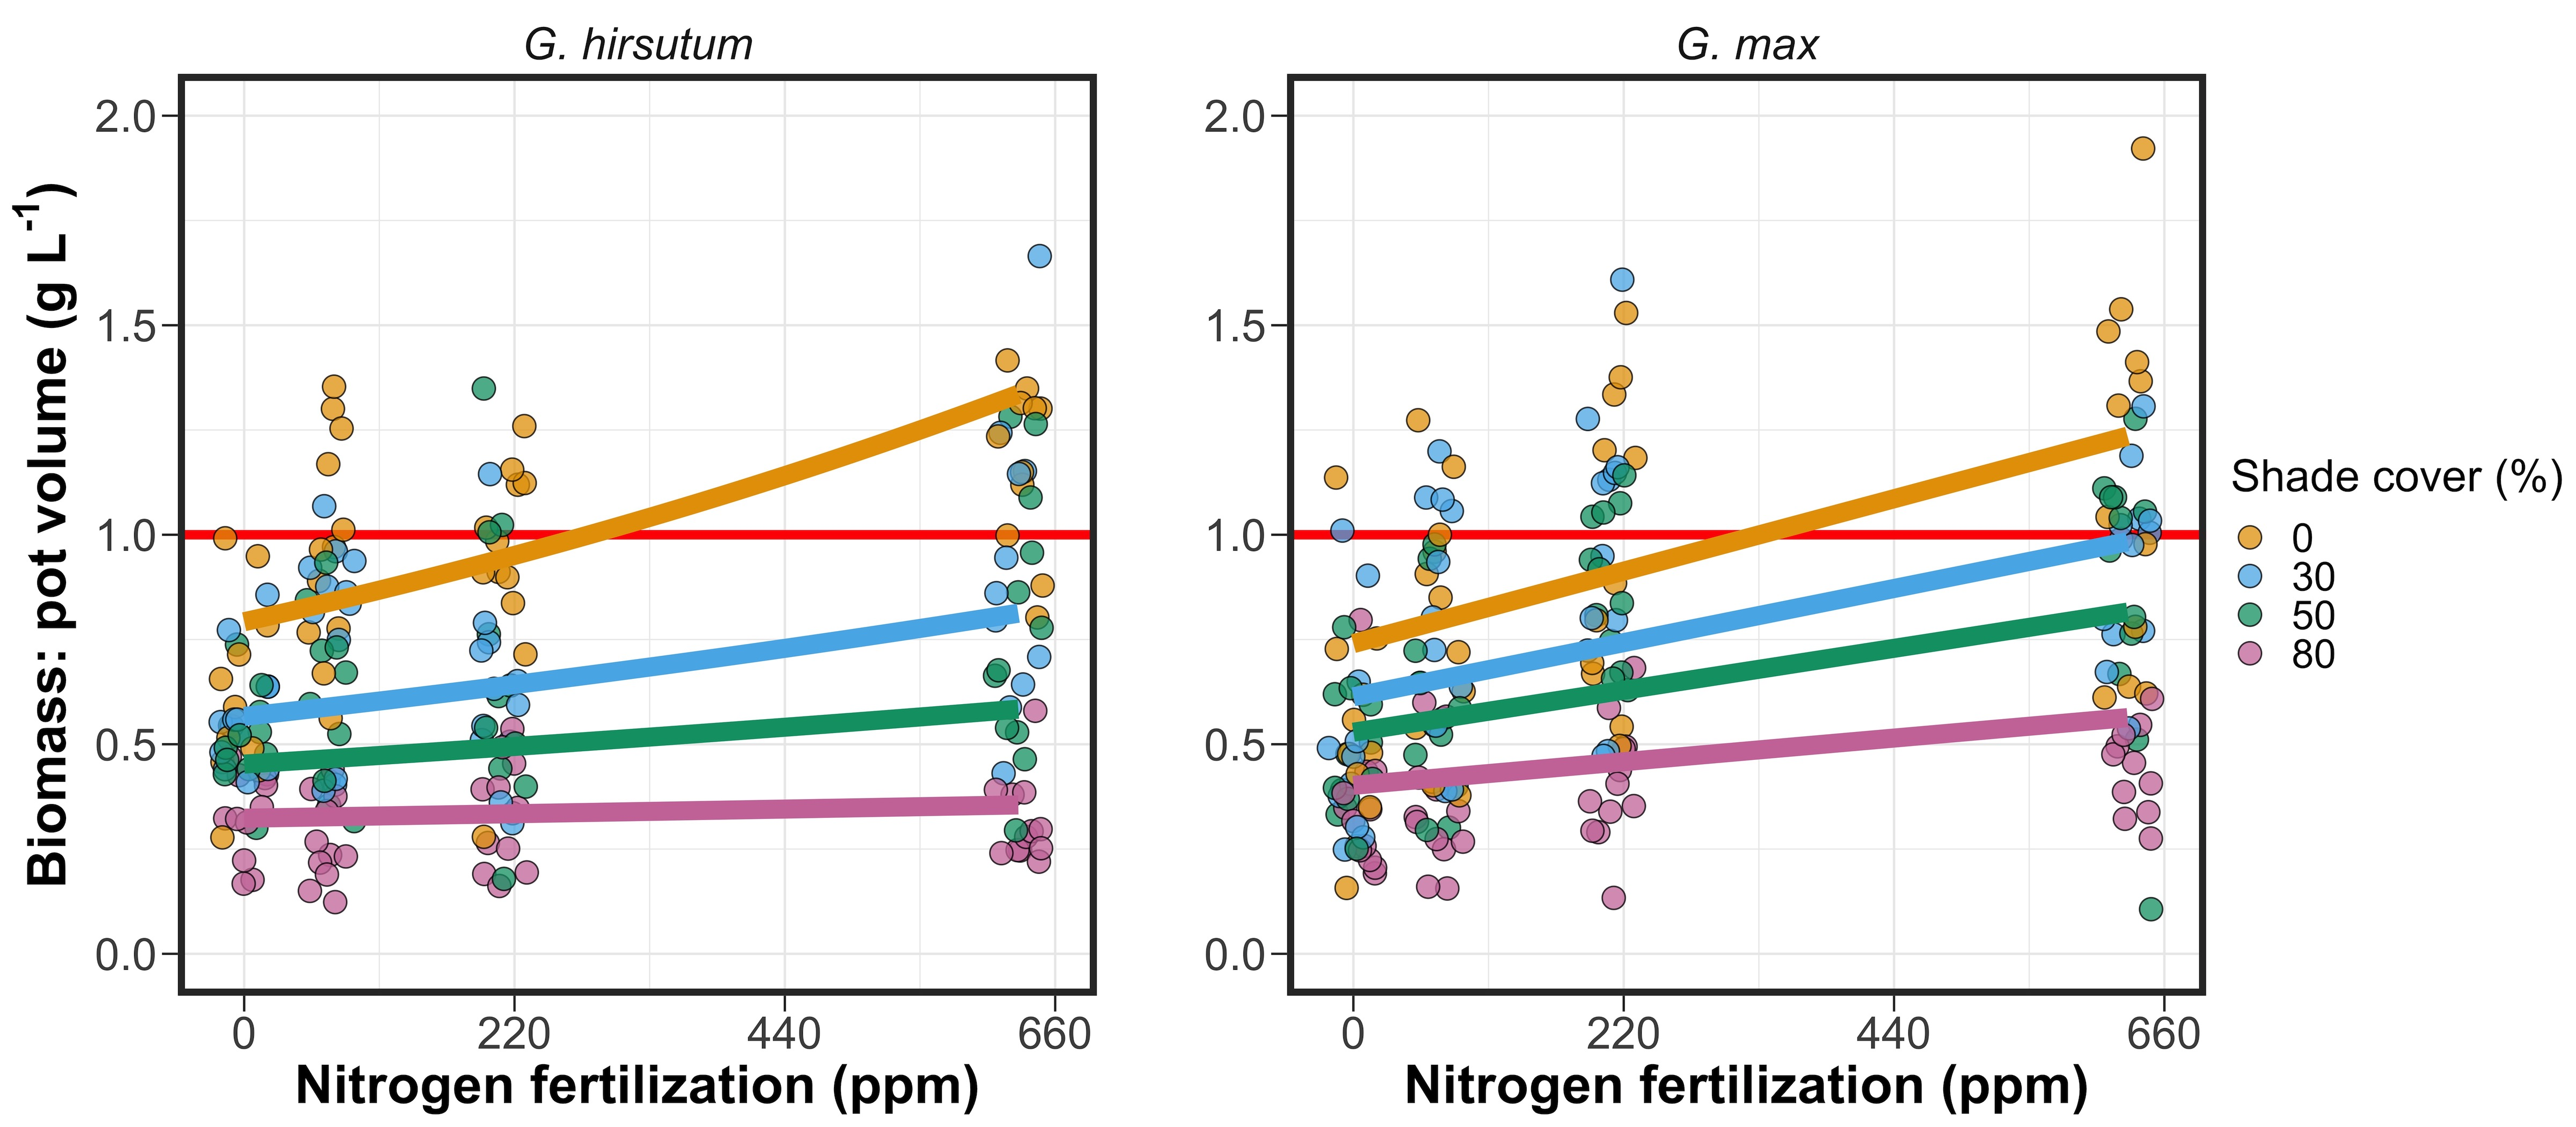
\includegraphics[width=\columnwidth]{ch2_LxN_Greenhouse/figs/figs1_bvr.jpg}
    \caption[Effects of shade cover and nitrogen fertilization on the ratio of plant biomass to rooting volume in \textit{G. hirsutum} and \textit{G. max}.]{Effects of shade cover and nitrogen fertilization on the ratio of plant biomass to rooting volume in \textit{G. hirsutum} (left panel) and \textit{G. max} (right panel). The red horizontal line indicates the recommended 1 g L$^{-1}$ threshold for biomass:pot volume recommended by \shortciteN{Poorter2012} to avoid pot size-induced growth limitation. Nitrogen fertilization treatments are represented on the x-axis. Shade cover treatments are represented through colored points and trendlines. Points are jittered for visibility. Yellow points and trendlines represent the 0\% shade cover treatment, blue points and trendlines represent the 30\% shade cover treatment, green points and trendlines represent the 50\% shade cover treatment, and purple points and trendlines represent the 80\% shade cover treatment. Solid trendlines indicate slopes that are significantly different from zero (Tukey: \textit{p}<0.05), while dashed trendlines indicate slopes that are not statistically different from zero.}
    \label{fig:figure.a1}
\end{figure}
\end{landscape}
\clearpage